\documentclass[11pt]{article}
\usepackage[margin=1in]{geometry}
\usepackage{amsmath,amssymb}
\usepackage{booktabs}
\IfFileExists{siunitx.sty}{\usepackage{siunitx}}{\def\NoSiunitx{1}}
\ifdefined\NoSiunitx
  \newcommand{\volt}{\mathrm{V}}\newcommand{\ampere}{\mathrm{A}}
  \newcommand{\ohm}{\Omega}
  \newcommand{\kilo}{\mathrm{k}}\newcommand{\milli}{\mathrm{m}}
  \newcommand{\micro}{\mu}\newcommand{\nano}{\mathrm{n}}
  \newcommand{\celsius}{{}^{\circ}\mathrm{C}}\newcommand{\second}{\mathrm{s}}
  \newcommand{\per}{/}
  \newcommand{\watt}{\mathrm{W}}
  \newcommand{\SI}[2]{\ensuremath{#1\,#2}}
  \newcommand{\SIrange}[3]{\ensuremath{#1\text{--}#2\,#3}}
\fi
\usepackage{enumitem}
\usepackage{graphicx}
\usepackage{xcolor}
\usepackage[colorlinks=true,linkcolor=blue,urlcolor=blue]{hyperref}

\newcommand{\Vref}{V_{\mathrm{REF}}}
\newcommand{\Vtlv}{V_{\mathrm{TLV}}}
\newcommand{\Vbe}{V_{\mathrm{BE}}}
\newcommand{\Vka}{V_{\mathrm{KA}}}
\newcommand{\Vout}{V_{OUT}}
\newcommand{\Vin}{V_{IN}}
\newcommand{\Varm}{V_{\mathrm{arm}}}
\newcommand{\uA}{\,\mu\mathrm{A}}
\newcommand{\vlo}{V_{BE}^{\mathrm{lo}}}
\newcommand{\vhi}{V_{BE}^{\mathrm{hi}}}

\title{UVLO Lockout Latch (rev.\ v3b): Discrete Pre-Bias Restart Protection\\
for the LM5176 Buck-Boost}
\author{USB-C PD $\to$ 12\,V Fan-Array Controller --- Buck-Boost 42\,W}
\date{}

\begin{document}
\maketitle

\begin{abstract}
\noindent
A four-BJT + TLV431 latch that pulls the LM5176 \texttt{EN/UVLO} pin low on an
input dropout and, because it is powered from $\Vout$, holds it low until the
output has discharged (release at $\approx$1.0--\SI{1.8}{\volt} across unit
tails), forcing every restart to begin from a nearly dead output. Rev.\ v3b uses a
\emph{ratio-defined} trigger --- v3's trigger depended on \emph{unspecified}
sub-threshold leakage; this one only on resistor ratios and spec'd $\Vbe$, so
it is consistent across part spread. The SCR core is armed by a resistor
divider (arm at \SI{2.8}{\volt} nominal, i.e.\ box-center $\Vbe$; guaranteed
range 2.0--\SI{3.6}{\volt}) and held off by an actively driven dearm
transistor while the TLV431 senses a healthy input (dearm active from
\SI{2.05}{\volt} worst case, \SI{27}{\milli\volt} of headroom above the
\SI{2.02}{\volt} physics floor). All device spreads are taken from the
\textbf{datasheet-box $\Vbe$ model} (traceable to the VBE(sat) spec), and the
dearm-before-arm race is guaranteed by those spec limits alone at every
temperature. Companion files: \texttt{10b\_uvlo\_latch.py} (all checks below,
executable), \texttt{uvlo\_tlv431.tex}/\texttt{10a} (EN/UVLO divider),
\texttt{simulation/en\_uvlo\_lockoutv3\_tlv.asc}.
\end{abstract}

\section{Background}

The LM5176's pre-bias startup does not survive a brief input dropout in this
design (deliberately slow control loop; TI support could not root-cause it).
The latch disables the converter on dropout and re-enables it only once the
output is discharged. Rev.\ v3 used Q3's sub-threshold leakage as the engage
seed; the required nA-level current is unspecified and spans orders of
magnitude across the 2N3904 spread and temperature. v3b moves the trigger onto
resistor ratios and spec'd $\Vbe$ --- robust and consistent by construction.

\section{The $\Vbe$ model (datasheet box, used everywhere below)}

Anchor: the 2N3904/2N3906 \textbf{VBE(sat) spec at $I_C=\SI{10}{\milli\ampere}$,
$I_B=\SI{1}{\milli\ampere}$, \SI{25}{\celsius}: 0.65 (min) .. 0.85 (max) V}.
The latch junctions operate near \SI{30}{\micro\ampere}, so the anchor is
scaled by the diode law $\Vbe=nV_T\ln(I_C/I_S)$ ($n\approx1$), whose
difference form removes the unknown $I_S$:
\[
\Vbe(I_1)-\Vbe(I_2)=V_T\ln\frac{I_1}{I_2}
\;\Rightarrow\;
\Delta\Vbe=25.9\,\mathrm{mV}\cdot\ln\frac{10\,\mathrm{mA}}{30\uA}
=25.9\times5.81=\SI{150}{\milli\volt},
\]
\[
\vlo(30\uA)=0.65-0.15=\SI{0.50}{\volt},\qquad
\vhi(30\uA)=0.85-0.15=\SI{0.70}{\volt}\quad(25\,{}^{\circ}\mathrm{C}),
\]
with the $-2\,\mathrm{mV/^{\circ}C}$ tempco applied for temperature (0--\SI{50}{\celsius}
design range: e.g.\ $\vhi(0\,\celsius)=0.75$, $\vlo(50\,\celsius)=0.45$).
\emph{Conservatism note:} VBE(sat) is a saturation measurement (both
junctions forward, base overdriven) and includes the ohmic drop $r_b I_B$
--- small-signal base spreading resistance is typically $r_b\approx10$--%
\SI{100}{\ohm}, i.e.\ 10--\SI{100}{\milli\volt} at the $I_B=\SI{1}{\milli
\ampere}$ test condition --- neither of which exists at
\SI{30}{\micro\ampere}. The true active-mode box is therefore narrower;
using the spec box as-is is the safe, traceable reading.

Other model values: $V_{CE,\mathrm{sat}}=0.1$ (max 0.2) V; $\beta_{\min}=30$;
$\Vbe^{\mathrm{off}}=\SI{0.4}{\volt}$ (design bound; ``off'' is defined
\emph{quantitatively} in step 2 --- leak $\ll$ hold drive --- not as zero);
$\Vka=1.24$ (max 1.27) V --- the latch's worst case is the \emph{max}, since
it sets the dearm floor; the corresponding \emph{min} is \SI{1.193}{\volt}
once the full onsemi $\Vka$ excursion is folded in
(\texttt{uvlo\_tlv431.tex}), which is what the divider search uses;
TLV431 (onsemi): $I_{K(\mathrm{off})}\le0.05\uA$,
$I_{KA}^{\mathrm{reg}}$ 30\,$\mu$A typ / 80\,$\mu$A max,
$I_K^{\max}=\SI{20}{\milli\ampere}$;
resistors $\pm3\%$ (1\% purchase $+$ $100\,\mathrm{ppm/^{\circ}C}$ tempco $+$
load-life/soldering drift); $\Vout$ = 12 nom / 15.75 max
(15\,V zener $+5\%$); $\Vin^{\max}=\SI{22}{\volt}$. EN/UVLO divider (sized in
\texttt{uvlo\_tlv431.tex}): $R_2/R_{1a}/R_{1b}=420/150/15\,\mathrm{k}\Omega$.

\section{Circuit and chosen values}

\begin{center}
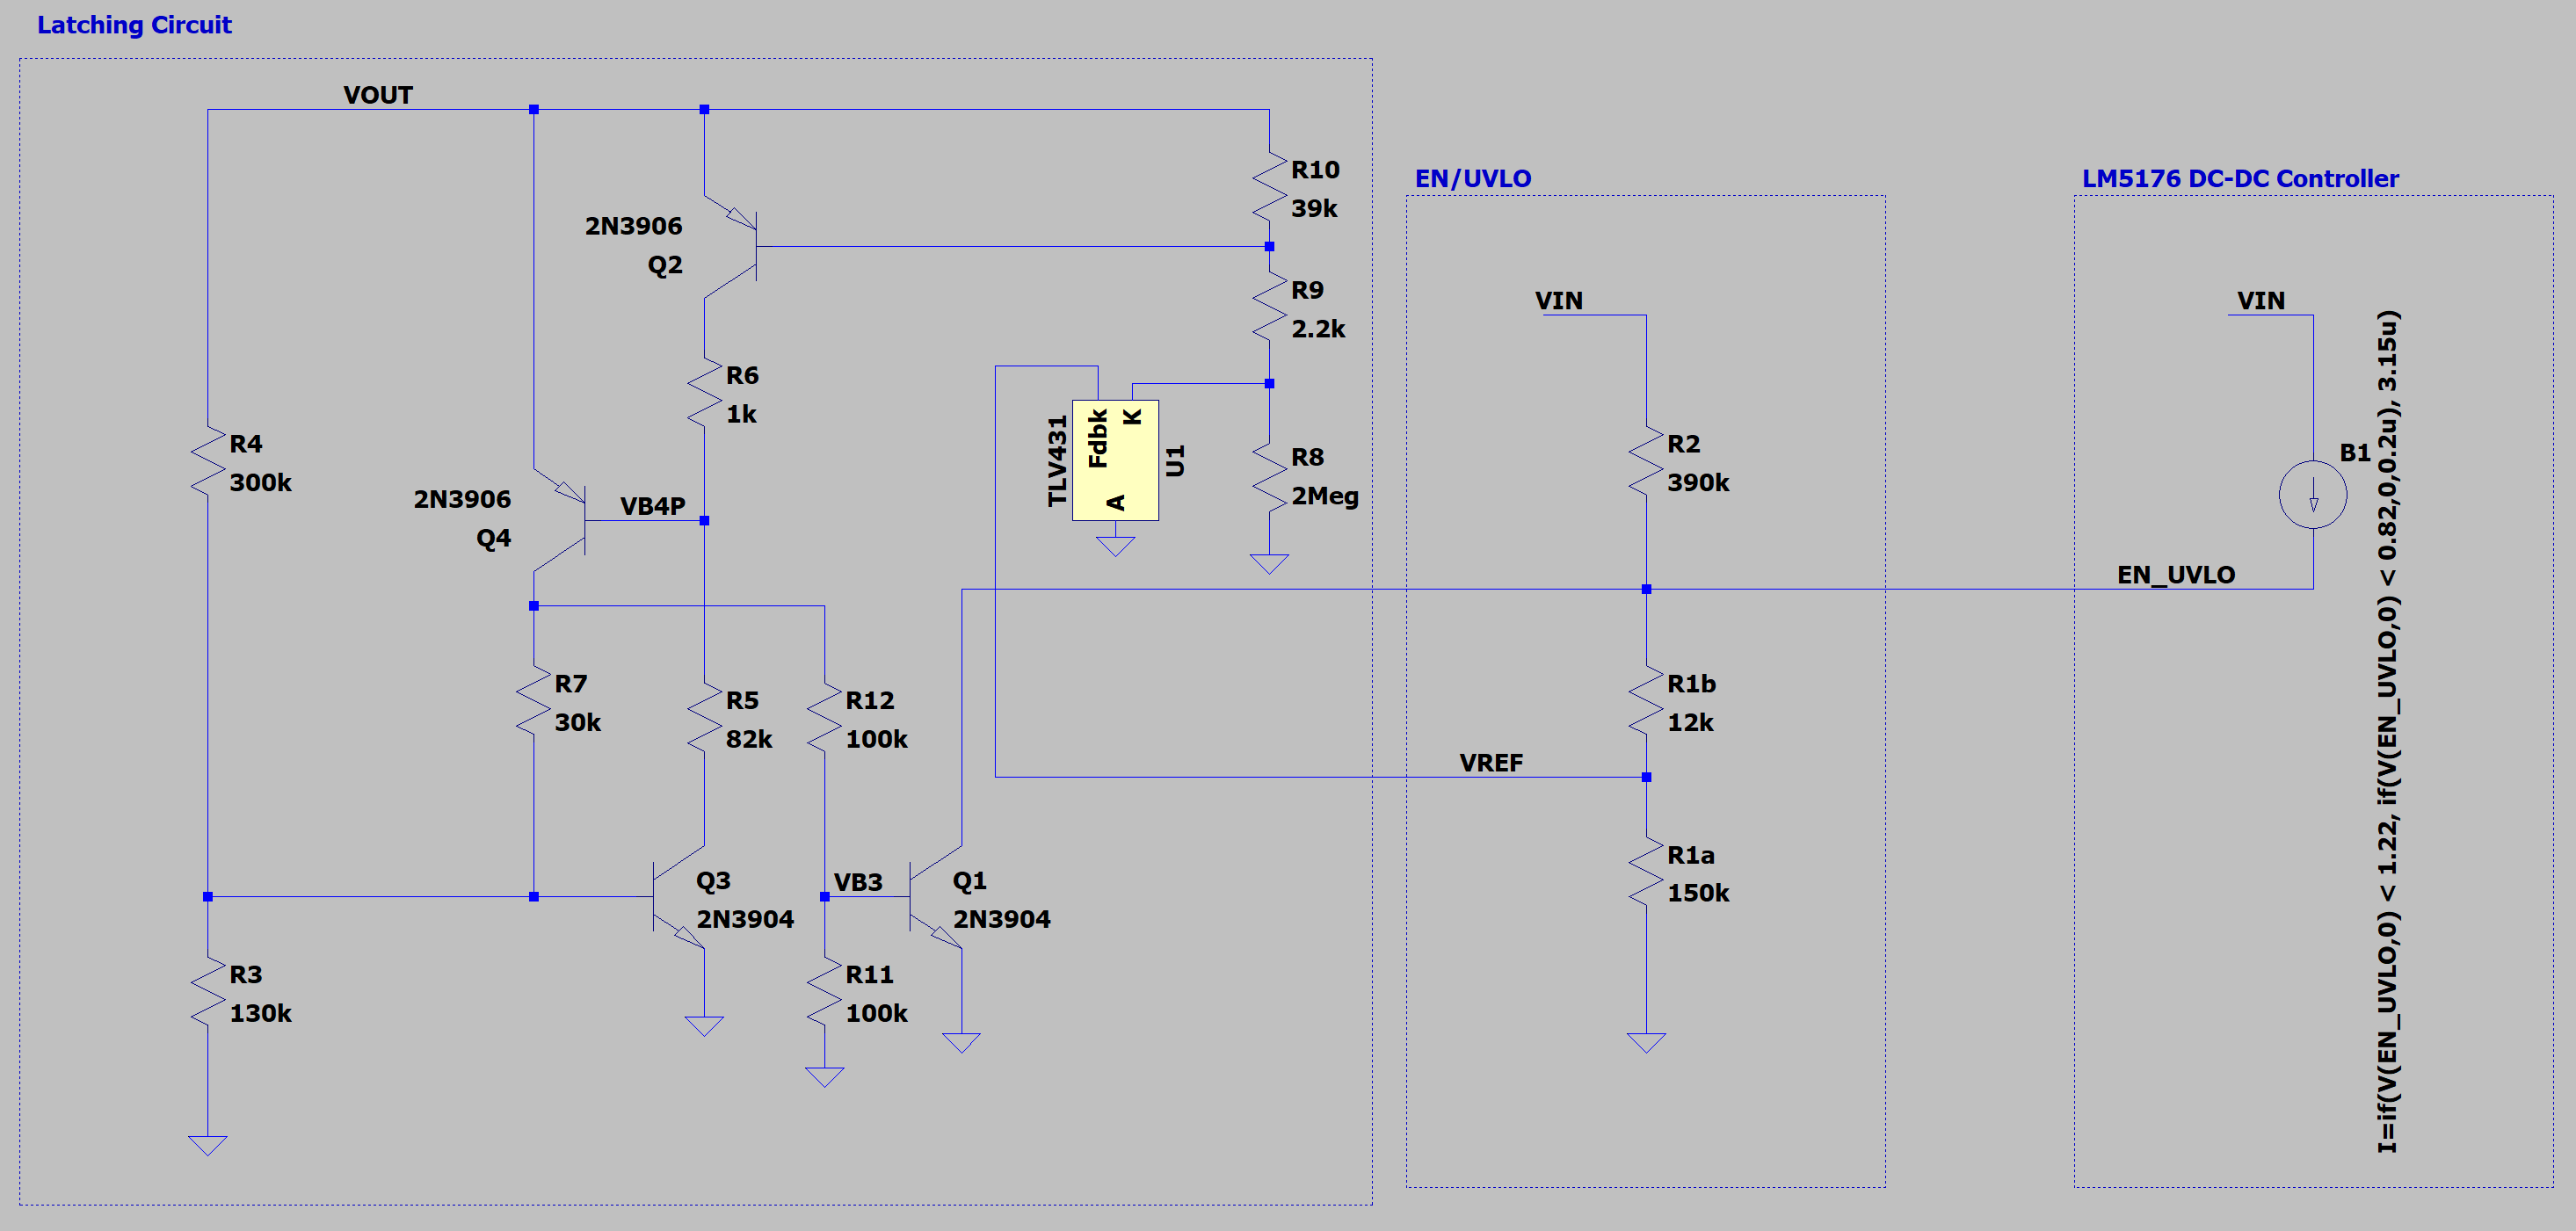
\includegraphics[width=\textwidth]{figures/divider_latch_schematic.png}
\end{center}
\noindent The latch is the left block; the \texttt{EN/UVLO} divider it senses
(and clamps) is on the right, sized in \texttt{uvlo\_tlv431.tex}.

\begin{center}
\begin{tabular}{llll}
\toprule
Ref & Value (bound $\to$ chosen) & Connection & Role \\
\midrule
Q1 & 2N3904 & c: \texttt{EN/UVLO}, b: N5, e: GND & EN clamp \\
Q2 & 2N3906 & e: $\Vout$, b: \texttt{VB2}, c: N1 & dearm driver \\
Q3 & 2N3904 & c: N4, b: \texttt{VB3}, e: GND & core NPN (armed switch) \\
Q4 & 2N3906 & e: $\Vout$, b: \texttt{VB4}, c: \texttt{VB1} & core PNP \\
R3 & race-solved $\le135\mathrm{k}\to$ \SI{130}{\kilo\ohm} & \texttt{VB3}--GND & arm divider bottom \\
R4 & \SI{300}{\kilo\ohm} (free choice) & $\Vout$--\texttt{VB3} & arm top / Q3 drive \\
R5 & $\ge 51 R_6\to$ \SI{82}{\kilo\ohm} & \texttt{VB4}--N4 & Q3 pulls Q4 base \\
R6 & \SI{1}{\kilo\ohm} & N1--\texttt{VB4} & Q2 pulls Q4 base up \\
R7 & \SI{30}{\kilo\ohm} & \texttt{VB1}--\texttt{VB3} & regeneration \\
R8 & tier choice (step 2) $\to$ \SI{2}{\mathrm{M}\ohm} & K--GND & TLV431 cathode load \\
R9 & window (step 1) $\to$ \SI{1.5}{\kilo\ohm} = $2\times$\SI{3}{\kilo\ohm} $\|$ (0603 pair) & \texttt{VB2}--K & Q2 base $\gets$ cathode \\
R10 & $\le\sim49\mathrm{k}$ solved (step 2) $\to$ \SI{47}{\kilo\ohm} & $\Vout$--\texttt{VB2} & Q2 base pull-up \\
R11 & \SI{100}{\kilo\ohm} & N5--GND & Q1 base divider bottom \\
R12 & \SI{100}{\kilo\ohm} & \texttt{VB1}--N5 & Q1 base divider top \\
U1 & TLV431 (\textbf{onsemi only}) & A: GND, K, REF: divider $\Vref$ & sensor \\
\bottomrule
\end{tabular}
\end{center}

Q3/Q4 with R5/R7 form the two-transistor SCR; Q1's base is driven from Q4's
collector through R12/R11, so before the latch fires its base sits at a
defined sub-threshold level (\SI{0.33}{\volt}, Stage 4) rather than floating
on leakage.

\section{Design walkthrough (sizing order, worked numbers)}

\subsection{Stage 1: R10, R9, R8 --- TLV431 sensing and the Q2 dearm driver}

\paragraph{Constraint set.} With the TLV431 regulating (K clamped at $\Vka$),
Q2's base drive is
\begin{equation}
I_{B2}=\frac{\Vout-\Vka-V_{EB2}}{R_9}-\frac{V_{EB2}}{R_{10}}
\;\ge\;I_{B2}^{\mathrm{req}}\approx1.1\uA
\quad\Longleftrightarrow\quad
R_{10}\;\ge\;\frac{V_{EB2}\,R_9}{h-R_9\,I_{B2}^{\mathrm{req}}},
\label{eq:dearm}
\end{equation}
with $h=\Vout-\Vka^{\max}-V_{EB2}$ the drive headroom; and with the TLV431 off,
\begin{equation}
V_{EB2}^{\mathrm{res}}=\Vout^{\max}\frac{R_{10}}{R_8+R_9+R_{10}}
+I_{K(\mathrm{off})}R_{10}\;\le\;\Vbe^{\mathrm{off}}=\SI{0.4}{\volt}.
\label{eq:resid}
\end{equation}
With $V_{EB2}=\vhi(0\,\celsius)=\SI{0.75}{\volt}$, the \textbf{physics floor}
is $\Vka^{\max}+V_{EB2}=1.27+0.75=\SI{2.02}{\volt}$.

\paragraph{Step 1: R9 from its independent bounds.}
R9 carries the full cathode current whenever the converter runs,
$I_K=(\Vout-V_{EB2}-\Vka)/R_9$, which is also the TLV431 regulation current:
\[
I_K\le\SI{20}{\milli\ampere}\text{ at }15.75\,\mathrm{V}:
\;R_9\ge\tfrac{13.81}{20\mathrm{m}}=\SI{0.69}{\kilo\ohm};\qquad
I_{KA}\ge80\uA\text{ at the box worst-low arm (\SI{1.98}{\volt}, step 3)}:
\;R_9\le\tfrac{1.98-1.24-0.65}{80\mu}\approx\SI{1.1}{\kilo\ohm}.
\]
Power: a \emph{single} 0805 would demand
$R_9\ge13.81^2/0.125=\SI{1.53}{\kilo\ohm}$, above the $I_{KA}$ bound: no
single resistor works. \textbf{Build $R_9=\SI{1.5}{\kilo\ohm}$ as two
\SI{3}{\kilo\ohm} basic 0603s in parallel} --- each part carries half the
current (\SI{34}{\milli\watt} continuous / \SI{64}{\milli\watt} at the OV
corner vs.\ 100\,mW rating). $I_{KA}$ razor: even 1.5\,k reads
$61\uA$ nominal / $59\uA$ at $R_9{+}3\%$ at the box-corner arm point vs the
$80\uA$ max-of-min --- reaching spec would need $R_9\le1.1$\,k, i.e.\ a
4-resistor array. Accepted: the shortfall exists only at the full R-corner +
hot + low-tail stack, fails soft (under-regulation raises K while $\Vout$ and
$I_{KA}$ keep rising), and typical parts need $30\uA$. Bench item for the
startup ramp. Why not smaller R9 (the headroom question):
\begin{center}
\begin{tabular}{lccccl}
\toprule
$R_9$ & dearm active & $I_K$@12\,V & $I_K$@15.75\,V & $P_{R9}$ tot @12/15.75\,V & verdict \\
\midrule
1.5\,k ($2{\times}3$k$\|$) & \SI{2.047}{\volt} & 6.7\,mA & 9.2\,mA & 67/127\,mW (34/64 per part) & \textbf{chosen} \\
1.0\,k ($2{\times}2$k$\|$) & \SI{2.038}{\volt} & 10.1\,mA & 13.8\,mA & 101/191\,mW & buys 9\,mV, $I_{KA}$ 91\,$\mu$A \\
0.5\,k & \SI{2.029}{\volt} & 20.1\,mA & 27.6\,mA & 202/381\,mW & exceeds 20\,mA rating \\
0.1\,k & \SI{2.022}{\volt} & 101\,mA & 138\,mA & 1.0/1.9\,W & $7\times$ over rating \\
\bottomrule
\end{tabular}
\end{center}

\paragraph{Step 2: pick the R8 tier, then SOLVE $R_{10}^{\max}$ from \eqref{eq:resid}.}
\eqref{eq:dearm} and \eqref{eq:resid} pull $R_{10}$ oppositely: larger $R_{10}$
lowers the dearm point (less bleed) but inflates the off-state residual, bought
back with larger $R_8$. The leakage term \emph{alone} would allow $R_{10}$ up
to $0.4/0.05\uA=\SI{8}{\mathrm{M}\ohm}$ --- nowhere near binding; the
divider term of \eqref{eq:resid} is what sets the bound. Basic-part $R_8$ above 510\,k comes only in 1\,M, 2\,M,
10\,M, so fix the tier and solve for $R_{10}$ (corners $R_{10}{+}3\%$,
$R_8,R_9{-}3\%$):
\begin{center}
\begin{tabular}{lcccc}
\toprule
$R_8$ tier & $R_{10}^{\max}$ solved & basic pick & dearm active & hot $I_{CBO}$(100\,nA)$\cdot R_{10}$ \\
\midrule
2\,M & $\sim$\SI{49}{\kilo\ohm} & \textbf{47\,k} & \SI{2.047}{\volt} & 4.7\,mV \\
10\,M & $\sim$\SI{230}{\kilo\ohm} & 220\,k & \SI{2.027}{\volt} & 22\,mV \\
\bottomrule
\end{tabular}
\end{center}
With $I_{K(\mathrm{off})}=50$\,nA the leakage term is negligible
($47\mathrm{k}\times50\,\mathrm{nA}=2.4$\,mV); the bound is the divider
alone. The 10\,M tier buys \SI{20}{\milli\volt} (asymptote
\SI{2.02}{\volt}) while quintupling $I_{CBO}$/board-leakage sensitivity ---
rejected. \textbf{Chosen: $R_8=\SI{2}{\mathrm{M}\ohm}$,
$R_{10}=\SI{47}{\kilo\ohm}$.} Verify \eqref{eq:resid} at corners
($R_{10}{+}3\%$, $R_8,R_9{-}3\%$):
$15.75\cdot\tfrac{48.4\mathrm{k}}{1.99\mathrm{M}}+50\mathrm{n}\cdot47\mathrm{k}
=0.383+0.002=\SI{0.386}{\volt}\le\SI{0.40}{\volt}$ \checkmark.
\emph{What ``off'' means, quantitatively:} at that residual, a box-worst
(low-tail, \SI{50}{\celsius}) Q2 still leaks
$I_{C2}=30\uA\cdot e^{(0.386-0.45)/V_T}=\SI{3.0}{\micro\ampere}$ --- but the
latch's VB4 hold drive at the same corner is \SI{183}{\micro\ampere}, so the
leak is 1.6\% of the hold: ``off'' means negligible against the hold, not
zero. The resulting worst-case \textbf{dearm-active point}: bleed
$=0.75/45.6\mathrm{k}=16.4\uA$,
$h=1.545\mathrm{k}\cdot(16.4{+}1.1)\uA=\SI{27}{\milli\volt}$
$\Rightarrow\Vout=\SI{2.05}{\volt}$ (a solved result, not a target; its only
requirement is the race, step 3).

\subsection{Stage 2 (step 3): R4, R3 --- the arm threshold and the race}

With Q4 off, \texttt{VB3} is loaded by R3 $\|$ (R7+R12+R11):
$R_3^{\mathrm{eff}}=130\|230=\SI{83.1}{\kilo\ohm}$, so
\begin{equation}
\Varm=\Vbe\Big(1+\frac{R_4}{R_3^{\mathrm{eff}}}\Big):\quad
\Varm^{\mathrm{mid}}=0.60\cdot4.61=\SI{2.77}{\volt},\quad
\Varm^{\min}=0.45\cdot4.40=\SI{1.98}{\volt},\quad
\Varm^{\max}=0.75\cdot4.84=\SI{3.63}{\volt},
\end{equation}
the ratio $1+R_4/R_3^{\mathrm{eff}}$ being evaluated at the $\pm3\%$ resistor
corners (4.40 / 4.61 / 4.84).
\textbf{R3 is solved from the race requirement:} dearm-active$(T)\le\Varm^{\min}(T)$
at every temperature, with Q2 at the box \emph{high} tail and Q3 at the box
\emph{low} tail simultaneously. The binding corner is \SI{50}{\celsius}:
$\Varm^{\min}\ge1.27+\vhi(50)+h=\SI{1.94}{\volt}$
$\Rightarrow R_3\le\SI{135}{\kilo\ohm}\to\SI{130}{\kilo\ohm}$ basic. Margins:
\[
\text{race margin}=\Varm^{\min}(T)-\text{dearm}(T)=
\SI{374}{\milli\volt}\,(0\,\celsius),\;\;
\SI{205}{\milli\volt}\,(25\,\celsius),\;\;
\SI{37}{\milli\volt}\,(50\,\celsius\ \text{binding}).
\]
Guaranteed by the datasheet box alone --- no unit screening required. Q3 drive
once armed: $I_{B3}=(\Vout-\Varm)/R_4\approx(12-2.77)/300\mathrm{k}=31\uA$
against the $142\uA$ dearm-chain load: forced $\beta=4.6\le10$.

\subsection{Stage 3 (step 4): R5, R6, R7 --- the VB4 fight and regeneration}

\textbf{Dearmed} (Q2 and Q3 both on): the chain
$\Vout\to Q2\to R_6\to R_5\to Q3\to$GND carries
$I=(\Vout-2V_{CE})/(R_5{+}R_6)$; \texttt{VB4} sits below $\Vout$ by
$V_{CE2}+I R_6$. At \SI{15.75}{\volt}: $I=15.55/83\mathrm{k}=187\uA$, so
$\Vout-V_{B4}=0.1+0.187=\SI{0.29}{\volt}\le\SI{0.40}{\volt}$ \checkmark
(this is where $R_5\ge51R_6$ comes from).
\textbf{Latched at the \SI{2}{\volt} hold floor} (cold tails: drive junctions
at $\vhi(0)=0.75$, loads at $\vlo(0)=0.55$):
$I_{B4}=(2-0.75-0.1)/82\mathrm{k}=14.0\uA$;
$I_{C4}=(1.9-0.55)(1/30\mathrm{k}+1/100\mathrm{k})=58.5\uA$: forced
$\beta=4.2$. Regeneration:
$I_{B3}=(1.9{-}0.75)/30\mathrm{k}+(2{-}0.75)/300\mathrm{k}-0.75/130\mathrm{k}
=38.3{+}4.2{-}5.8=36.7\uA$ against a $14\uA$ load.

\subsection{Stage 4 (step 5): R12, R11 --- the Q1 EN clamp}

Off before the latch fires: $V_{N5}=\vhi(0)\cdot R_{11}/(R_7{+}R_{12}{+}R_{11})
=0.75\cdot100/230=\SI{0.33}{\volt}$, below even a hot low-tail unit's
\SI{0.45}{\volt} conduction. Clamp at the \SI{2}{\volt} hold floor:
$I_{B1}=(1.9-0.75)/100\mathrm{k}-0.75/100\mathrm{k}=4.0\uA$ against the
requirement $I_{EN}/\beta_{\min}=57.6\uA/30=1.9\uA$: margin $2.1\times$.
Release, solving $I_{B1}=I_{EN}/\beta$:
\begin{equation}
\Vout^{\mathrm{rel}}=V_{CE4}+\Vbe+R_{12}\Big(\frac{I_{EN}}{\beta}
+\frac{\Vbe}{R_{11}}\Big)
=\SI{1.05}{\volt}\ (\vlo,\Vin{=}6)\;\ldots\;\SI{1.79}{\volt}\ (\vhi,\Vin{=}22).
\end{equation}
Hold \emph{guaranteed} at \SI{2.0}{\volt}; \emph{actual} release 1.0--1.8\,V by
unit; the SCR core itself un-latches near \SI{0.8}{\volt}.

\section{Operating sequence (summary)}

\begin{enumerate}[nosep]
\item Cold start: $\Vout=0$, latch unpowered, Q1 base defined low.
\item $\Vout$ rises: dearm active from \SI{2.05}{\volt} (worst), arm at
      2.0--\SI{3.6}{\volt}; dearm wins by $\ge$\SI{37}{\milli\volt} at any
      single temperature, guaranteed by the datasheet box.
\item Dropout with $\Vout>\Varm$: TLV off $\to$ Q2 off $\to$ Q3 wins
      \texttt{VB4} $\to$ Q4 on $\to$ Q1 clamps EN; R7 regenerates.
\item EN low $\Rightarrow\Vref\le0.19$\,V $\ll\Vtlv$: hold is $\Vin$-proof.
\item $\Vout$ decays; EN releases at 1.0--\SI{1.8}{\volt}; clean restart.
\end{enumerate}

\paragraph{Accepted gap.} A dropout while $\Vout$ is between release
(1.0--1.8\,V) and that unit's arm point (2.0--3.6\,V) does not latch. More
precisely: the latch cannot act \emph{anywhere} below its arm point, so the
unprotected region is $\Vout<\Varm$ --- it extends down to zero, not merely to
the release point. (The release point governs when an \emph{already engaged}
latch lets go; it is not a lower bound on the exposure.)

Two qualifications matter. First, body diodes do not bound it: the LM5176
switches synchronously, so an enabled FET conducts in either direction.
Second --- and this is the part that makes the exposure a safety question --- a
stored-energy argument does not bound it. A passive dump through a conducting
FET would simply equalise the two banks at
$\Vout C_{OUT}/(C_{OUT}{+}C_{IN})=\SI{3.56}{\volt}$, which is harmless. But a
buck-boost transfers \emph{energy} through its inductor, and the input bank is
$90\times$ smaller ($C_{OUT}\approx\SI{18.9}{\milli\farad}$ vs.\
$C_{IN}\approx\SI{0.21}{\milli\farad}$), so any reverse transfer is a boost
into a small capacitor:
\begin{equation}
V_{IN}\;\approx\;\Vout\sqrt{\frac{C_{OUT}}{C_{IN}}}
\;=\;3.6\times9.5\;\approx\;\SI{34}{\volt},
\end{equation}
against a \SI{22}{\volt} operating maximum and \SI{35}{\volt} input
electrolytics --- with the attached USB source seeing the same rail. Even a
quarter of the energy arriving gives $\approx\SI{17}{\volt}$.

\emph{Open item (safety).} Confirm by bench and simulation that the LM5176's
pre-biased startup performs no reverse energy transfer for $\Vout$ below the
arm point. Until that is shown the low-$\Vout$ band is an accepted, documented
exposure; the case for extending protection below the arm point --- or for
clamping the input --- rests on that measurement.

\section{TLV431 vendor constraint}

Eliminating the resistors from \eqref{eq:dearm}/\eqref{eq:resid} gives the floor
$V_K^{\mathrm{worst}}\ge V_{OUT}^{\max}-\tfrac{\Vbe^{\mathrm{off}}}{V_{EB2}}
(V_{\mathrm{dearm}}-\Vka)=15.75-\tfrac{0.4}{0.75}(2.05-1.24)=\SI{15.3}{\volt}$;
the chosen divider gives $15.75\cdot2\mathrm{M}/2.05\mathrm{M}=\SI{15.4}{\volt}$.
Holding $V_K\le\SI{6}{\volt}$ is therefore impossible at any useful dearm
point, which is why the design assumes the onsemi TLV431
($\Vka^{\max}=\SI{16}{\volt}$) rather than the pin-compatible TI part. The
\SI{15.4}{\volt} figure is itself a double-fault corner: K only floats high
while the latch is engaged, and in that state $\Vout$ is decaying from
$\approx$12.6\,V, giving a realistic $V_K\approx\SI{12.4}{\volt}$.

\section{Quiescent draw}

Dearmed at \SI{12}{\volt}: R9 chain $\tfrac{12-0.7-1.24}{1.5\mathrm{k}}=6.7$\,mA
$+$ R10 $15\uA$ $+$ R5{+}R6 $142\uA$ $+$ R4 $31\uA$ $\approx\SI{6.9}{\milli\ampere}$
($\approx\SI{83}{\milli\watt}$). Each 3\,k of the R9 pair dissipates
\SI{34}{\milli\watt} continuous / \SI{64}{\milli\watt} at the OV corner
(0603-safe). This is the price of the \SI{2.05}{\volt} dearm point.

\section{Verification status}

\texttt{10b\_uvlo\_latch.py} runs the above as 21 worst-case checks: 0 FAIL,
2 WARN (the 59--$61\uA$ $I_{KA}$ razor of step 1, and the onsemi-only vendor
note), and parses the latest \texttt{.raw}.

The current LTspice transient (schematic at R3 = 130k, R5 = 82k, R8 = 2M,
R9 = 2.2k, R10 = 39k, EN/UVLO divider already at the recommended
420/150/15\,k$\Omega$, plus a behavioural EN-pin current source:
\SI{0.2}{\micro\ampere} below threshold, \SI{3.15}{\micro\ampere} enabled)
confirms the full sequence:
\begin{itemize}[nosep]
\item \textbf{Arm:} \texttt{VB3} clamps at \SI{0.64}{\volt} --- Q3 on, core armed.
\item \textbf{Engage:} EN clamps at $\Vin=\SI{3.47}{\volt}$ vs.\
      \SI{3.51}{\volt} predicted from the divider equation at
      $\Vtlv=1.24$, $I_S=\SI{3.15}{\micro\ampere}$ (1.3\,\% error).
\item \textbf{Hold:} EN $\le\SI{10}{\milli\volt}$ through a full $\Vin$
      re-application at $\Vout=\SI{12}{\volt}$.
\item \textbf{Release:} at $\Vout=\SI{1.08}{\volt}$, inside the predicted
      1.0--\SI{1.8}{\volt} band.
\item \textbf{Dearmed:} $\Vref=\SI{1.88}{\volt}$ while running
      ($>\Vtlv=\SI{1.24}{\volt}$), i.e.\ the TLV431 conducts throughout
      normal operation as C2/C3 require.
\end{itemize}
The simulated circuit still carries two intermediate values, $R_9=$
\SI{2.2}{\kilo\ohm} (vs.\ the \SI{1.5}{\kilo\ohm} of the $2\times3$\,k pair)
and $R_{10}=$ \SI{39}{\kilo\ohm} (vs.\ \SI{47}{\kilo\ohm}). Both final values
only \emph{lower} the worst-case dearm point (2.09 $\to$ \SI{2.05}{\volt}), so
the sequence above is representative of the final design.

\begin{center}
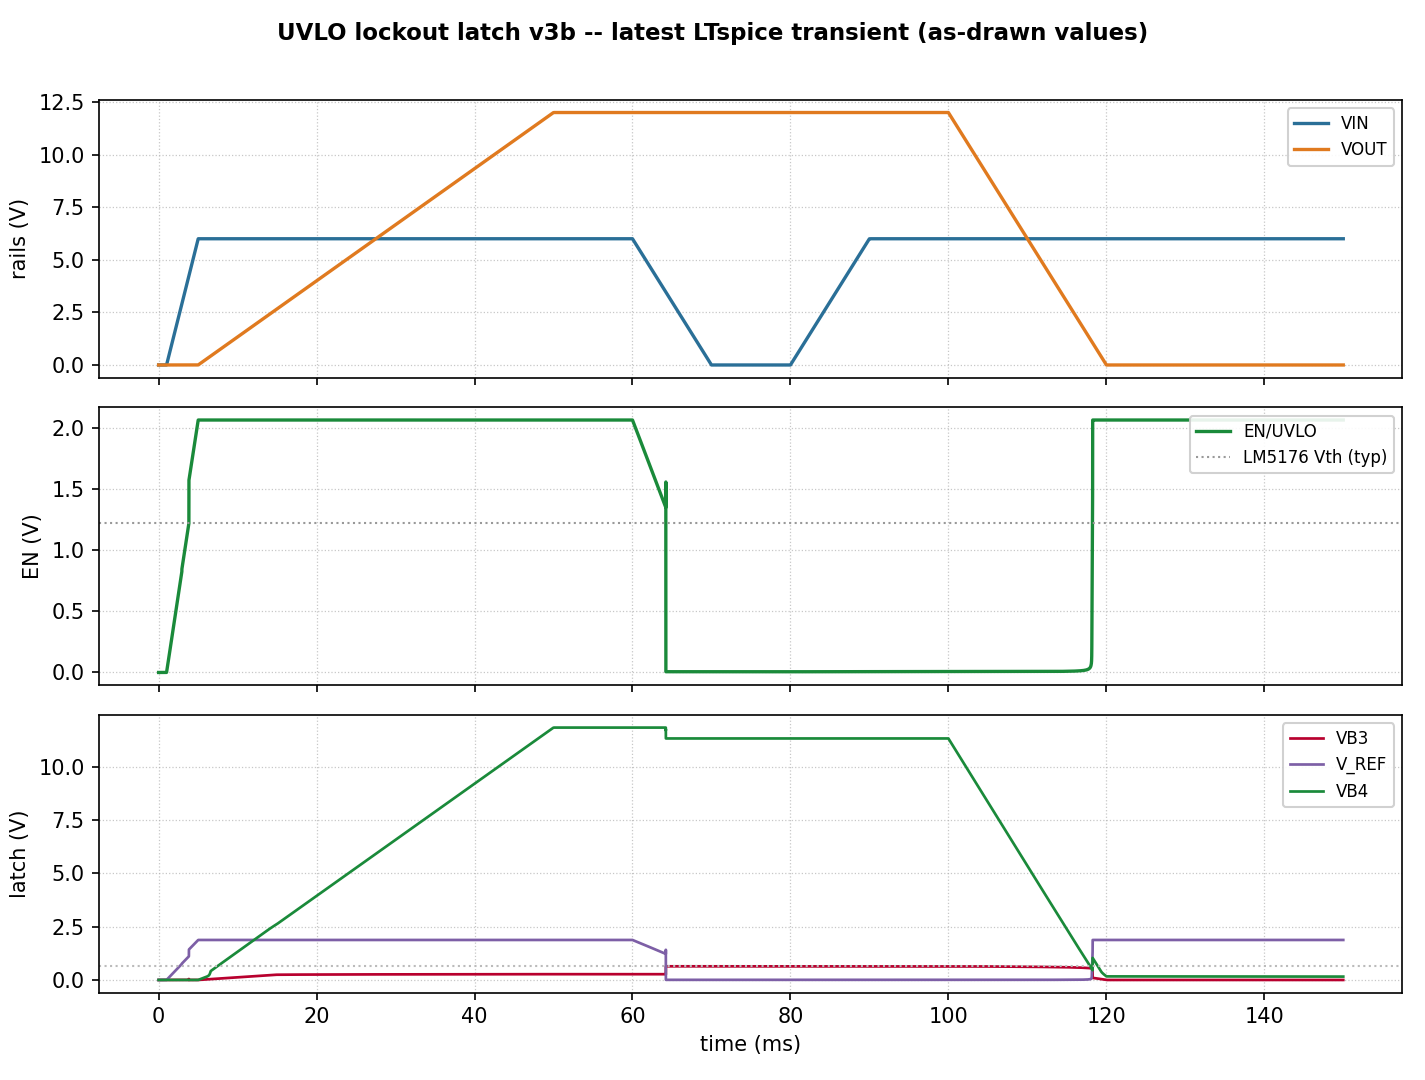
\includegraphics[width=\textwidth]{figures/uvlo_latch_sim.png}
\end{center}

\end{document}
